%【紙面設定】
%b4,横書き,2段
\documentclass[paper=b4j,landscape,twocolumn,fleqn]{jlreq}
\special{papersize=\the\paperwidth,\the\paperheight}
\setlength{\columnseprule}{0.4pt}
\pagestyle{empty}

\usepackage[margin=8truemm]{geometry}
\usepackage[dvipdfmx]{graphicx}
\usepackage{amsmath,amssymb}
\usepackage{tikz}
\usetikzlibrary{arrows.meta,calc}

\ModifyHeading{section}{
  lines=1,
  before_space=6pt,
  after_space=0pt
}

\setlength{\parskip}{0pt}
\setlength{\jot}{3pt}

\newcommand{\blank}[1]{\underline{\rule[-0.2em]{0pt}{1.4em}\hspace{#1}}}

\begin{document}
\normalsize

\section{ベクトルとは何か}
\begin{align*}
&\text{量だけを表すものを }\blank{2.0cm}\text{ という。}\\[0.5em]
&\text{量と向きをあわせて表すものを }\blank{2.0cm}\text{ という。}\\[0.5em]
&\text{等しいベクトルの条件は「}\blank{2.4cm}\text{ と }\blank{2.4cm}\text{ が同じ」ことである。}
\end{align*}

\textbf{右の図において、次のベクトルと等しいものを $a\sim f$ から選べ。}
\begin{center}
\begin{minipage}[t]{0.46\columnwidth}
\vspace{0pt}
\begin{align*}
&(1)\ \vec{a}\text{ と等しいベクトル}\\[0.6em]
&(2)\ \vec{b}\text{ と等しいベクトル}\\[0.6em]
&(3)\ \vec{e}\text{ と等しいベクトル}
\end{align*}
\end{minipage}\hfill
\begin{minipage}[t]{0.50\columnwidth}
\vspace{0pt}
\centering
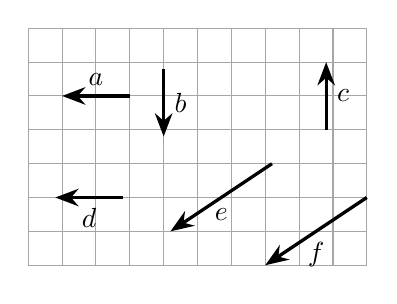
\begin{tikzpicture}[scale=0.43,>=Stealth]
  \draw[step=1,gray!70] (0,0) grid (10,7);
  \draw[very thick,->] (3,5) -- (1,5) node[midway,above] {$a$};
  \draw[very thick,->] (4,5.8) -- (4,3.8) node[midway,right] {$b$};
  \draw[very thick,->] (8.8,4.0) -- (8.8,6.0) node[midway,right] {$c$};
  \draw[very thick,->] (2.8,2.0) -- (0.8,2.0) node[midway,below] {$d$};
  \draw[very thick,->] (7.2,3.0) -- (4.2,1.0) node[midway,below] {$e$};
  \draw[very thick,->] (10.0,2.0) -- (7.0,0.0) node[midway,below] {$f$};
\end{tikzpicture}
\end{minipage}
\end{center}

\vspace{6pt}
\section{成分表示・大きさ・単位ベクトル}
\noindent
\begin{tabular*}{\columnwidth}{@{\extracolsep{\fill}}p{0.47\columnwidth}p{0.49\columnwidth}@{}}
\vspace{0pt}
\[
\begin{aligned}
\vec{a}&=\begin{pmatrix}a_x & a_y\end{pmatrix}について考える。\\[1.4em]
|\vec{a}|&=\sqrt{\blank{1.8cm}+\blank{1.8cm}}\\[1.4em]
\hat{a}&=\dfrac{\fbox{\rule[-0.6em]{0pt}{1.8em}\hspace{2.2cm}}}{\fbox{\rule[-0.6em]{0pt}{1.8em}\hspace{2.2cm}}}\qquad|\hat{a}|=\blank{2.0cm}
\end{aligned}
\]
&
\vspace{0pt}\centering
\resizebox{0.98\linewidth}{!}{%
\begin{tikzpicture}[scale=0.84,>=Stealth]
  \draw[->,gray!60] (-0.3,0) -- (5.8,0) node[right] {$x$};
  \draw[->,gray!60] (0,-0.3) -- (0,4.8) node[above] {$y$};
  \draw[very thick,blue,->] (0,0) -- (4.2,3.2) node[midway,below right] {$\vec{a}$};
  \draw[dashed,gray!70] (4.2,0)--(4.2,3.2);
  \draw[dashed,gray!70] (0,3.2)--(4.2,3.2);
  \node[draw,very thick,minimum width=0.95cm,minimum height=0.55cm] at (-0.85,3.2) {};
  \node[draw,very thick,minimum width=0.95cm,minimum height=0.55cm] at (4.2,-0.55) {};
  \node[right] at (4.35,3.55) {$\left(\blank{0.8cm}\ \blank{0.8cm}\right)$};
\end{tikzpicture}
}
\end{tabular*}

\vspace{6pt}
\section{足し算・引き算・スカラー倍}
\noindent
\begin{tabular*}{\columnwidth}{@{\extracolsep{\fill}}p{0.47\columnwidth}p{0.49\columnwidth}@{}}
\vspace{0pt}
\[
\begin{aligned}
\begin{pmatrix}a_x & a_y\end{pmatrix}+\begin{pmatrix}b_x & b_y\end{pmatrix}
&=\begin{pmatrix}\blank{1.2cm} & \blank{1.2cm}\end{pmatrix}\\[1.1em]
\begin{pmatrix}a_x & a_y\end{pmatrix}-\begin{pmatrix}b_x & b_y\end{pmatrix}
&=\begin{pmatrix}\blank{1.2cm} & \blank{1.2cm}\end{pmatrix}\\[1.1em]
k\begin{pmatrix}a_x & a_y\end{pmatrix}
&=\begin{pmatrix}\blank{1.2cm} & \blank{1.2cm}\end{pmatrix}\\[1.1em]
-k\begin{pmatrix}a_x & a_y\end{pmatrix}
&=\begin{pmatrix}\blank{1.2cm} & \blank{1.2cm}\end{pmatrix}
\end{aligned}
\]
&
\vspace{0pt}\centering
\resizebox{0.98\linewidth}{!}{%
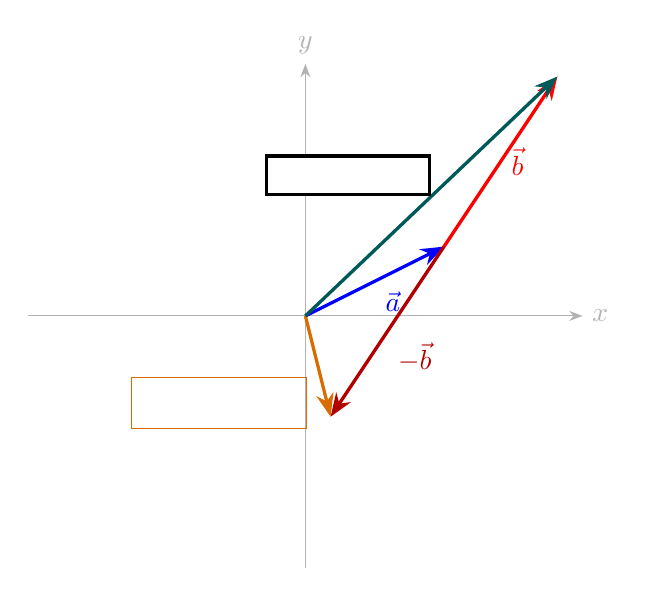
\begin{tikzpicture}[scale=0.8,>=Stealth]
  \draw[->,gray!60] (-4.4,0) -- (4.4,0) node[right] {$x$};
  \draw[->,gray!60] (0,-4.0) -- (0,4.0) node[above] {$y$};
  \draw[very thick,blue,->] (0,0)--(2.2,1.1) node[midway,below right] {$\vec{a}$};
  \draw[very thick,red,->] (2.2,1.1)--(4.0,3.8) node[midway,right] {$\vec{b}$};
  \draw[very thick,red!70!black,->] (2.2,1.1)--(0.4,-1.6) node[midway,below right] {$-\vec{b}$};
  \draw[very thick,orange!85!black,->] (0,0)--(0.4,-1.6) node[midway,below left] {$\fbox{\rule[-0.45em]{0pt}{1.2em}\hspace{2.0cm}}$};
  \draw[very thick,teal!70!black,->] (0,0)--(4.0,3.8)
    node[midway,above left,fill=white,draw=black,inner sep=1pt] {$\rule[-0.45em]{0pt}{1.2em}\hspace{2.0cm}$};
\end{tikzpicture}
}
\end{tabular*}

\newpage

\section{内積と角度}
\noindent
\begin{tabular*}{\columnwidth}{@{\extracolsep{\fill}}p{0.48\columnwidth}p{0.48\columnwidth}@{}}
\vspace{0pt}
\begin{minipage}[t]{\linewidth}
\vspace{0pt}
\[
\begin{aligned}
\vec{a}&=\begin{pmatrix}a_x & a_y\end{pmatrix},\quad \vec{b}=\begin{pmatrix}b_x & b_y\end{pmatrix}\\[1.0em]
&成分計算：\vec{a}\cdot\vec{b}=\blank{4.4cm}\\[0.5em]
&なす角計算：\vec{a}\cdot\vec{b}=\blank{1.1cm}\blank{1.1cm}\blank{1.5cm}\\[0.5em]
&\cos\theta=\dfrac{\fbox{\rule[-0.6em]{0pt}{1.8em}\hspace{2.2cm}}}{\fbox{\rule[-0.6em]{0pt}{1.8em}\hspace{2.2cm}}}\\[0.5em]
&\vec{a}\cdot\vec{b}=0\iff\vec{a}と\vec{b}は\blank{1.4cm}
\end{aligned}
\]
\end{minipage}
&
\vspace{0pt}\hspace*{0cm}
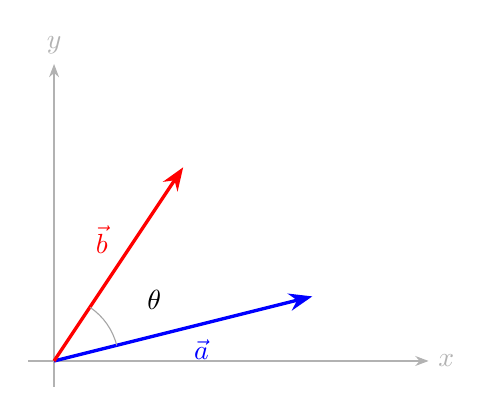
\begin{tikzpicture}[scale=0.82,>=Stealth]
  \draw[->,gray!60] (-0.4,0) -- (5.8,0) node[right] {$x$};
  \draw[->,gray!60] (0,-0.4) -- (0,4.6) node[above] {$y$};
  \coordinate (O) at (0,0);
  \coordinate (A) at (4.0,1.0);
  \coordinate (B) at (2.0,3.0);
  \draw[very thick,blue,->] (O)--(A) node[midway,below right] {$\vec{a}$};
  \draw[very thick,red,->] (O)--(B) node[midway,above left] {$\vec{b}$};
  \draw[gray!70] (14:1.0) arc[start angle=14,end angle=56,radius=1.0];
  \node at (1.55,0.95) {$\theta$};
\end{tikzpicture}
\end{tabular*}

\vspace{30pt}
\section{2次元の外積と面積}
\noindent
\begin{tabular*}{\columnwidth}{@{\extracolsep{\fill}}p{0.48\columnwidth}p{0.48\columnwidth}@{}}
\vspace{0pt}
\begin{minipage}[t]{\linewidth}
\vspace{0pt}
\[
\begin{aligned}
\vec{a}&=\begin{pmatrix}a_x & a_y\end{pmatrix},\quad \vec{b}=\begin{pmatrix}b_x & b_y\end{pmatrix}\\[1.0em]
&\vec{a}\times\vec{b}=\blank{3.8cm}\\[0.5em]
&\vec{a}\times\vec{b}=-(\blank{2.6cm})\\[0.5em]
&\text{外積の結果が+：}\blank{1.4cm}\\[0.4em]
&\text{外積の結果が-：}\blank{1.4cm}\\[0.5em]
&\text{平行四辺形の面積}=\blank{2.2cm}
\end{aligned}
\]
\end{minipage}
&
\vspace{0pt}\hspace*{0cm}
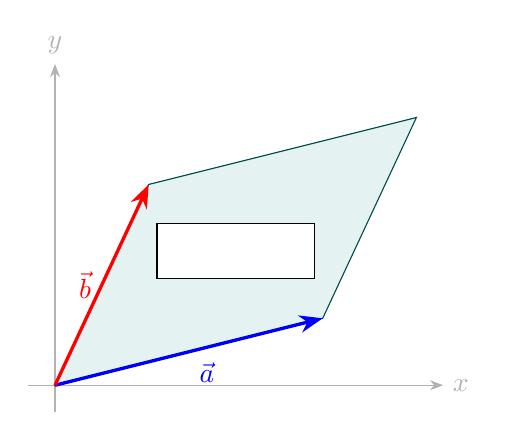
\begin{tikzpicture}[scale=0.85,>=Stealth]
  \draw[->,gray!60] (-0.4,0) -- (5.8,0) node[right] {$x$};
  \draw[->,gray!60] (0,-0.4) -- (0,4.8) node[above] {$y$};
  \coordinate (O) at (0,0);
  \coordinate (A) at (4,1);
  \coordinate (B) at (1.4,3.0);
  \coordinate (C) at ($(A)+(B)$);
  \filldraw[fill=teal!10,draw=teal!60!black] (O)--(A)--(C)--(B)--cycle;
  \node[draw=black,fill=white,minimum width=2.0cm,minimum height=0.7cm,inner sep=0pt] at ($(O)!0.5!(C)$) {};
  \draw[very thick,blue,->] (O)--(A) node[midway,below right] {$\vec{a}$};
  \draw[very thick,red,->] (O)--(B) node[midway,left] {$\vec{b}$};
\end{tikzpicture}
\end{tabular*}

\vspace{8pt}
\section{射影}
\noindent
\begin{tabular*}{\columnwidth}{@{\extracolsep{\fill}}p{0.48\columnwidth}p{0.48\columnwidth}@{}}
\vspace{0pt}
\begin{minipage}[t]{\linewidth}
\vspace{0pt}
\[
\begin{aligned}
&\text{手順1：}\hat{b}=\dfrac{\fbox{\rule[-0.6em]{0pt}{1.8em}\hspace{2.2cm}}}{\fbox{\rule[-0.6em]{0pt}{1.8em}\hspace{2.2cm}}}\qquad|\hat{b}|=\blank{2.0cm}\\[0.6em]
&\text{手順2：}\vec{a}\cdot\hat{b}=|\vec{a}|*|\hat{b}|*\cos\theta=|\vec{a}|*\blank{0.8cm}*\cos\theta\\[0.3em]
&\hspace{3.9em}=\blank{2.2cm}=|\vec{A}|\\[0.6em]
&\text{手順3：}\vec{A}=\hat{b}*\blank{0.8cm} = \hat{b}*(\vec{a}\cdot\hat{b})\\[0.6em]
\end{aligned}
\]
\begin{center}
よって、\blank{1.0cm}から\blank{1.0cm}への射影ベクトルは\\
\vspace{8pt}
{\Large $\vec{A}=\hat{b}*(\vec{a}\cdot\hat{b})$}
\end{center}
\end{minipage}
&
\vspace{0pt}\hspace*{0cm}
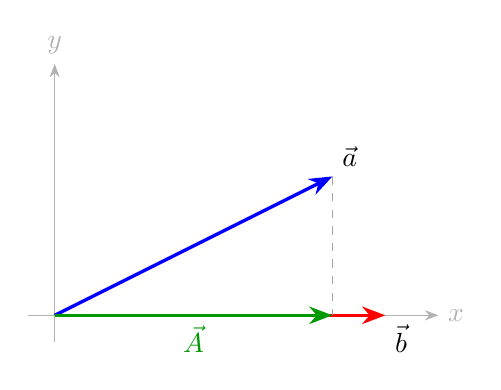
\begin{tikzpicture}[scale=0.84,>=Stealth]
  \draw[->,gray!60] (-0.4,0) -- (5.8,0) node[right] {$x$};
  \draw[->,gray!60] (0,-0.4) -- (0,3.8) node[above] {$y$};
  \coordinate (O) at (0,0);
  \coordinate (A) at (4.2,2.1);
  \coordinate (P) at (4.2,0);
  \draw[very thick,blue,->] (O)--(A);
  \node[above right] at (A) {$\vec{a}$};
  \draw[very thick,red,->] (O)--(5.0,0);
  \node[below right] at (5.0,0) {$\vec{b}$};
  \draw[dashed,gray!70] (A)--(P);
  \draw[very thick,green!60!black,->] (O)--(P) node[midway,below] {$\vec{A}$};
\end{tikzpicture}
\end{tabular*}

\end{document}
